\documentclass[a0paper,portrait,fontscale=0.285]{baposter}

\usepackage{lmodern}
\usepackage{graphicx}
\usepackage[utf8]{inputenc}
\usepackage[T1]{fontenc}
\usepackage{amsmath}
\usepackage{booktabs}
\usepackage{enumitem}
\usepackage{tabularx}
\usepackage{tikz}
\usetikzlibrary{arrows.meta, positioning, calc}
\usepackage{fontawesome5}
\usepackage{pdfrender}

%\selectcolormodel{cmyk} % disabled: caused colour shift vs standalone figures (RGB)

\graphicspath{{./}}

\newcommand{\sectionnum}[1]{%
  \raisebox{0pt}[0pt][0pt]{%
    \makebox[1.4em][c]{%
      \textcolor{white}{\textsf{\textbf{\Large #1}}}%
    }%
  }\hspace{0.3em}%
}

\begin{document}

\definecolor{posternavy}{HTML}{1B2A4A}
\definecolor{posterborder}{HTML}{00857C}
\definecolor{boxbg}{HTML}{FAFAFA}
\definecolor{coneRed}{HTML}{C62828}
\definecolor{drivcol}{HTML}{7AB648}
\definecolor{impcol}{HTML}{C62828}
\definecolor{droughttan}{HTML}{D4A574}
\definecolor{floodblue}{HTML}{4A90D9}

% Outlined + filled text: white stroke with coloured fill
\newcommand{\outlinedtext}[2]{% #1=fill colour, #2=text
  \textpdfrender{TextRenderingMode=FillStroke,LineWidth=0.4pt,StrokeColor=white,FillColor=#1}{#2}%
}

\begin{poster}
{
grid=false,
headerborder=none,
colspacing=0.7em,
margin=2.5cm,
bgColorOne=white,
bgColorTwo=white,
borderColor=posternavy,
headerColorOne=posternavy,
headerColorTwo=posternavy,
headerFontColor=white,
boxColorOne=boxbg,
textborder=rounded,
eyecatcher=false,
headerheight=0.113\textheight,
headershape=rounded,
headershade=plain,
headerfont=\Large\textsf,
linewidth=0.8pt,
background=plain
}
{} % eyecatcher (disabled)
{% Title
\color{white}\sffamily
{\fontsize{26}{32}\selectfont\bfseries
Towards Subseasonal-to-Seasonal\\[0.15em]
\outlinedtext{droughttan}{Drought}\hspace{0.15em}{\color{white}-to-}\hspace{0.15em}\outlinedtext{floodblue}{Flood} Prediction}\\[0.4em]
{\large\mdseries \textbf{Lainey Ward}\textsuperscript{1}, Fiachra O'Loughlin\textsuperscript{1}, Conor Sweeney\textsuperscript{2}}\\[0.2em]
{\small\mdseries \textsuperscript{1}School of Civil Engineering, \textsuperscript{2}School of Mathematics and Statistics, University College Dublin}
}
{} % author (unused, content is in title block)
{% Right logos — raisebox to top-align with title text
\raisebox{5.3em}{
\includegraphics[height=3.8em]{ucd.png}\hspace{1.2em}%

\includegraphics[height=3.8em]{IFICOPY.png}}\hspace{0.2em}%
}

%----------------------------------------------------------------------
% ROW 1: 1 — Introduction (full width)
%----------------------------------------------------------------------
\headerbox{Introduction}{name=introduction,column=0,row=0.012,span=3}{
\begin{tikzpicture}[remember picture, overlay]
\node[anchor=north east] at ([xshift=-0.7cm, yshift=-2.5cm]current page.north east)
    {
\includegraphics[height=1.8cm]{qrcode_linkedin.png}};
\end{tikzpicture}%

\noindent
\begin{minipage}[t]{0.45\linewidth}
\vspace{0pt}
Floods and droughts can occur in sequence --- a \textbf{\textcolor{impcol}{drought-to-flood transition (DFT)}}. Globally, \textbf{$\sim$25\% of floods are preceded by drought} [2], and socio-economic losses can be up to \textbf{8x greater} than from isolated hazards [3]. Forecasting DFTs at subseasonal-to-seasonal (S2S) lead times could support early action, but 2 research gaps remain\,\,$\longrightarrow$
\end{minipage}%
\hfill
\begin{minipage}[t]{0.51\linewidth}
\vspace{0pt}
\begin{tikzpicture}[
    gapbox/.style={
        rectangle, rounded corners=3pt, line width=1.0pt,
        fill=black!4, minimum height=0.9em, text width=4.8cm,
        align=center, font=\sffamily, inner xsep=5pt, inner ysep=3pt
    },
    goalbox/.style={
        rectangle, rounded corners=3pt, line width=1.1pt,
        fill=black!4, minimum height=1.0em, text width=3.8cm,
        align=center, font=\sffamily\bfseries, inner xsep=5pt, inner ysep=4pt
    },
    arrow/.style={
        -{Stealth[length=6pt, width=5pt]}, line width=1.4pt, color=black!70
    },
    thiswork/.style={
        font=\sffamily\bfseries, text=drivcol!80!black,
        draw=drivcol!70, fill=drivcol!8, rounded corners=2pt,
        inner xsep=3pt, inner ysep=1.5pt
    },
]
\node[gapbox, draw=posternavy!70]
    (gap2) at (-1.5, 0.8)
    {No catalogue of DFT\\events exists for Ireland};
\node[thiswork]
    (marker) at (-1.5, 0)
    {$\downarrow$\, Current focus};
\node[gapbox, draw=drivcol!80!black, dashed]
    (gap1) at (-1.5, -0.8)
    {S2S forecast skill over\\Ireland has not been assessed};
\node[goalbox, draw=impcol!80!black, right=3.2cm of marker]
    (goal)
    {S2S DFT\\prediction};
\draw[arrow] (gap2.east) to[out=0, in=180] (goal.west);
\draw[arrow] (gap1.east) to[out=0, in=180] (goal.west);
\path (-3.5, 0) -- (-3.5, 0); % extend bounding box left to shift diagram right
\end{tikzpicture}
\end{minipage}

\vspace{0.3em}

\noindent
\begin{minipage}[c]{0.82\linewidth}
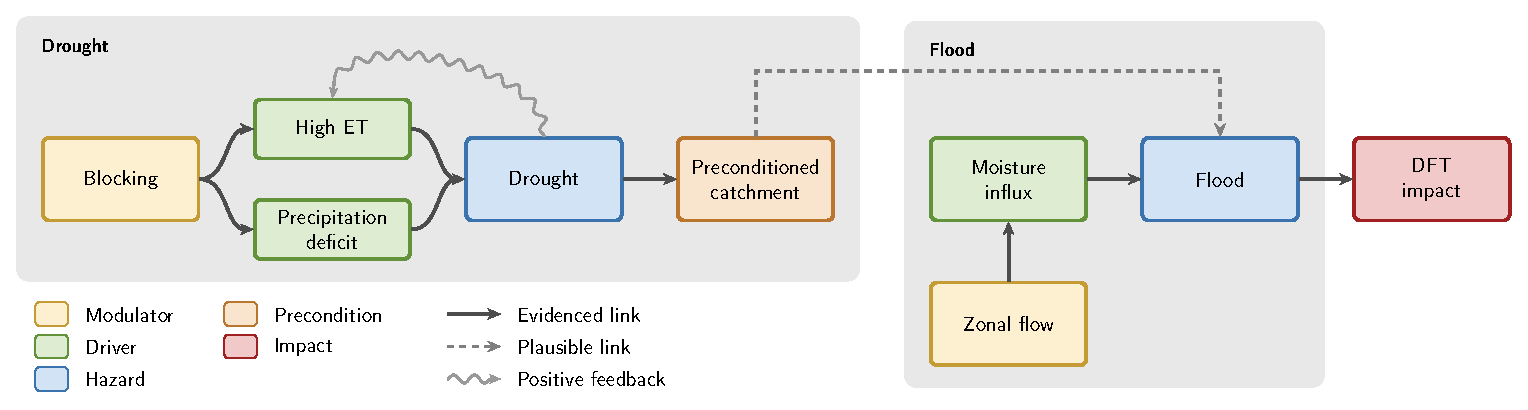
\includegraphics[width=\linewidth]{dft_causal_diagram_poster.pdf}
\end{minipage}%
\hfill
\begin{minipage}[c]{0.16\linewidth}
\raggedright
{\small \textbf{Figure 1:} Physical pathway for DFT events, after the framework of Bevacqua et~al.\ [1].}
\end{minipage}
}

%----------------------------------------------------------------------
% ROW 2 LEFT: 3 — Methods (defined first so Data can bottomalign to it)
%----------------------------------------------------------------------
\headerbox{Methods}{name=methods,column=0,below=introduction,span=2}{

We verify 2\,m temperature forecasts at \textbf{2--6 week} lead times, pooling all reforecast initialisations (2005--2024) per season and lead. Two complementary metrics are used: \textbf{Fair CRPSS} (Continuous Ranked Probability Skill Score) [4], scored against ERA5 climatology, and \textbf{centred ACC} (Anomaly Correlation Coefficient). Mean bias is removed by leave-one-year-out correction.

\vspace{1.2em}

\newlength{\accboxwidth}
\setlength{\accboxwidth}{\dimexpr\linewidth-1.0em\relax}% inner text width
\noindent
\begin{tikzpicture}
\node[draw=drivcol!80!black, fill=drivcol!10, rounded corners=6pt, line width=0.8pt,
      inner sep=0.5em, text width=\accboxwidth] {%
\begin{minipage}[c]{0.62\accboxwidth}
$\displaystyle
\text{ACC} \;=\; \frac{\displaystyle\sum_{m=1}^{M} w_m\,(f'_m - \bar{f}'\,)(o'_m - \bar{o}'\,)}{\left[\displaystyle\sum_{m=1}^{M} w_m\,(f'_m - \bar{f}'\,)^{2}\;\cdot\;\sum_{m=1}^{M} w_m\,(o'_m - \bar{o}'\,)^{2}\right]^{1/2}}
$
\end{minipage}%
\hfill
\begin{minipage}[c]{0.35\accboxwidth}
{\footnotesize
\begin{tabular}{@{}r@{\;=\;}l@{}}
$f'_m,\; o'_m$ & forecast/observed anomalies \\
$\bar{f}',\; \bar{o}'$ & area-weighted spatial means \\
$w_m$ & $\cos\varphi$ (latitude weight) \\
$M$ & number of gridpoints \\
\end{tabular}

\vspace{0.3em}
\hfill{\scriptsize Wilks (2011), Eq.~7.59\; [5]}
}
\end{minipage}%
};
\end{tikzpicture}
\vspace{-0.9em}
}

%----------------------------------------------------------------------
% ROW 2 RIGHT: 2 — Data
%----------------------------------------------------------------------
\headerbox{Data}{name=data,column=2,below=introduction,span=1,bottomaligned=methods}{

\begin{center}
{\small
\renewcommand{\arraystretch}{1.3}
\begin{tabular}{@{}rl@{}}
\textbf{System} & ECMWF ENS extended-range \\
\textbf{IFS cycle} & CY49R1 (2024) \\
\textbf{Init.\ freq.} & Every 2 days \\
\textbf{Members} & 11 (1 control + 10 perturbed) \\
\textbf{Horizon} & Weeks 2--6 \\
\textbf{Variable} & 2\,m temperature \\
\textbf{Grid} & 0.28\textdegree{} regular lat-lon (MARS) \\
\textbf{Reference} & ERA5 + Met \'Eireann stations \\
\textbf{Reforecasts} & 2005--2024 \\
\end{tabular}
}
\end{center}

}

%----------------------------------------------------------------------
% ROW 3: 4 — Results (full width)
%----------------------------------------------------------------------
\headerbox{Results}{name=results,column=0,below=methods,span=3}{

\noindent
\begin{minipage}[t]{0.48\linewidth}
\vspace{0pt}
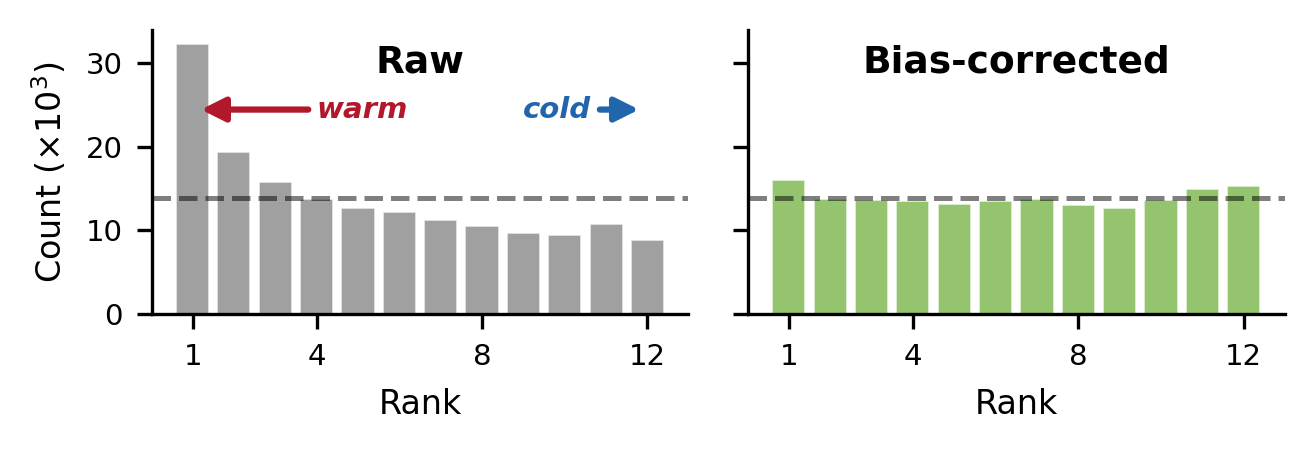
\includegraphics[width=\linewidth]{poster_fig_rankhist.png}\\[-0.3em]
{\small \textbf{Figure 2:} Rank histograms before/after seasonal LOYO bias correction.}

\vspace{0.3em}

\noindent
\begin{minipage}[c]{0.58\linewidth}
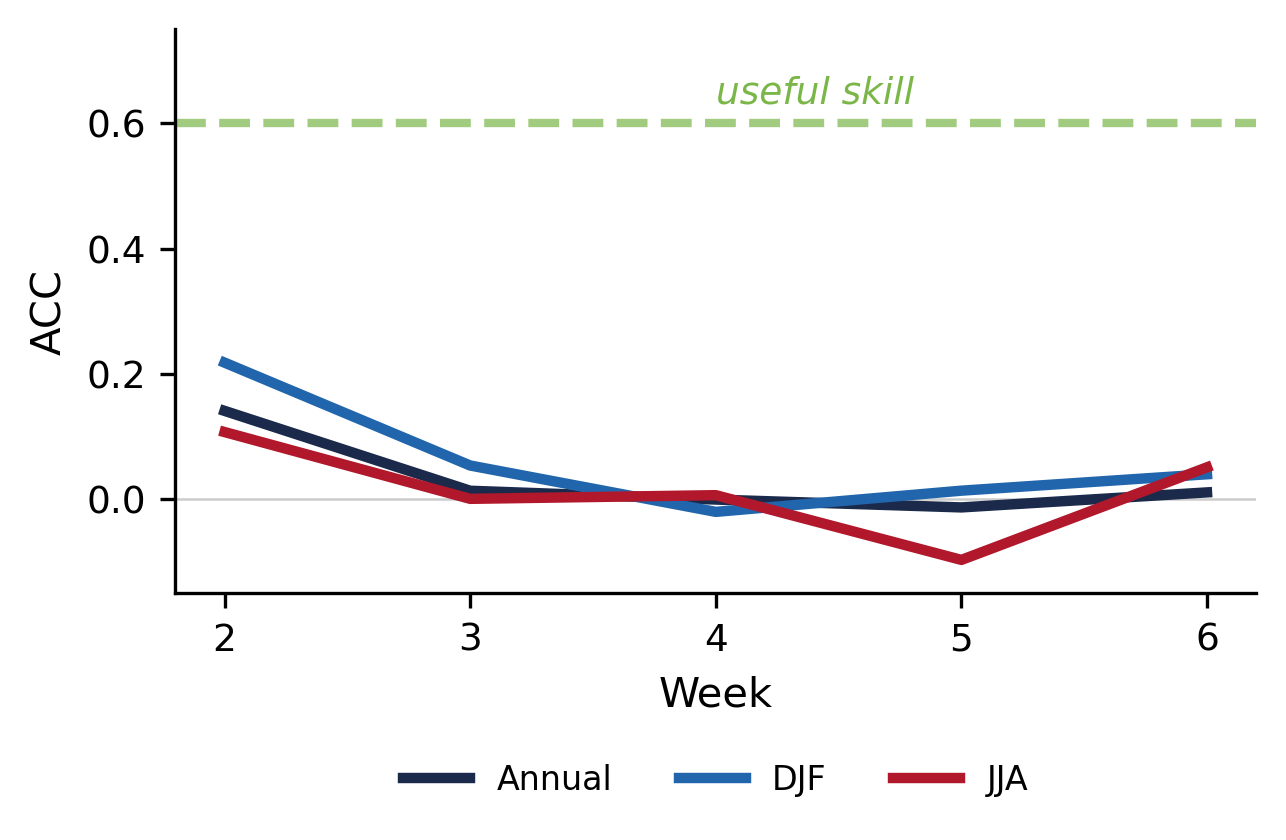
\includegraphics[width=\linewidth]{poster_fig_acc.png}
\end{minipage}%
\hfill
\begin{minipage}[c]{0.38\linewidth}
{\small \textbf{Figure 3:} ACC vs lead time.}
\end{minipage}
\end{minipage}%
\hfill
\begin{minipage}[t]{0.48\linewidth}
\vspace{0pt}
\raggedleft
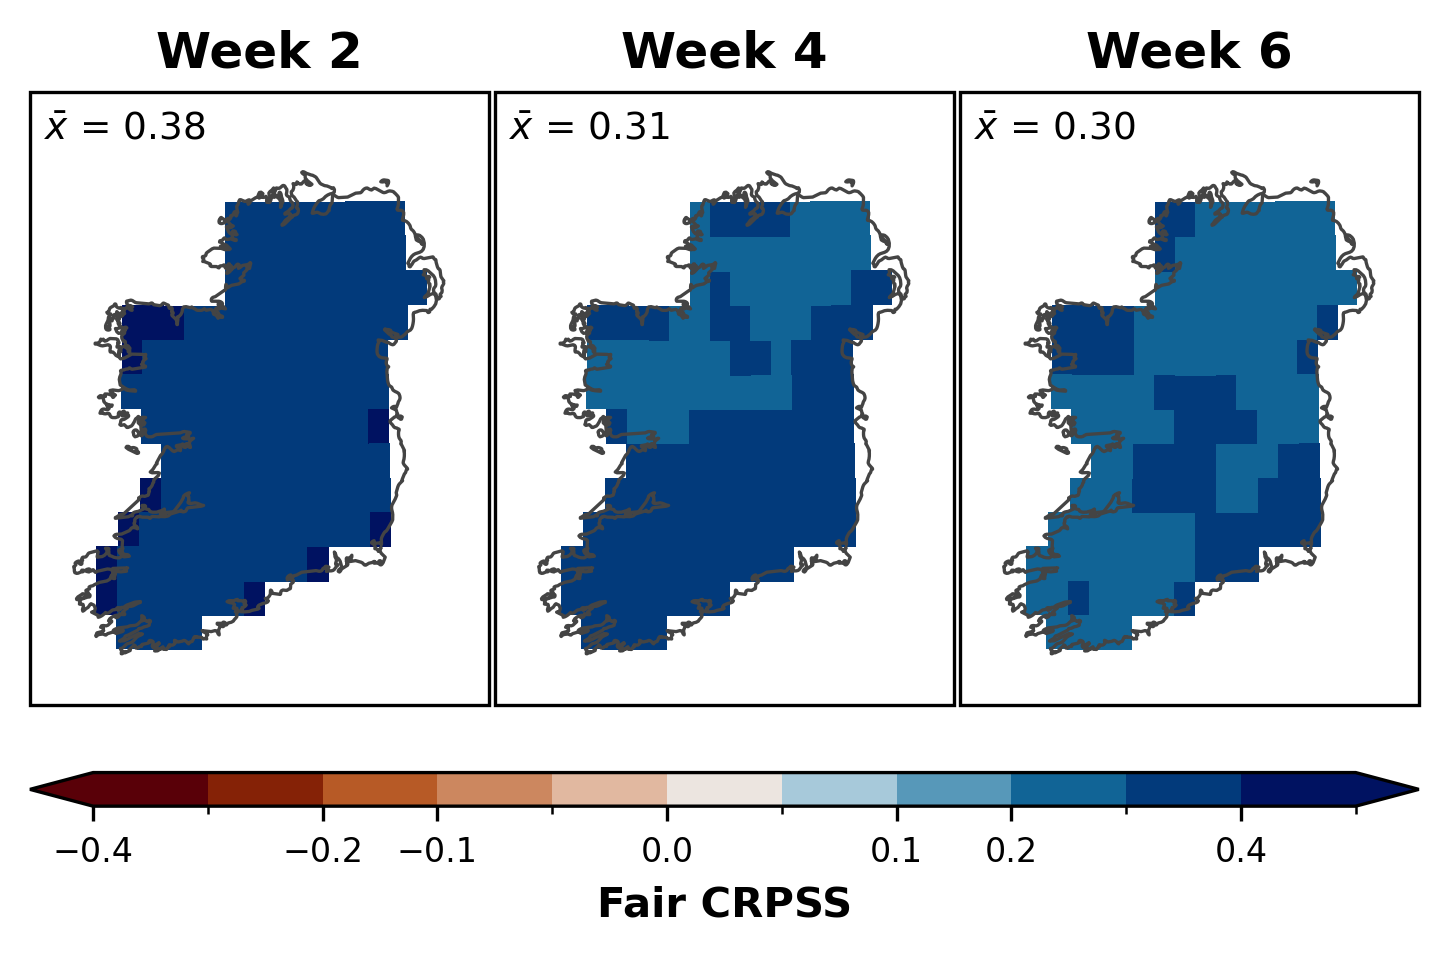
\includegraphics[width=0.85\linewidth]{poster_fig_crpss.png}\\[0.1em]
\hfill\parbox{0.92\linewidth}{\raggedright\small \textbf{Figure 4:} Fair CRPSS across lead time (bias-corrected).}
\end{minipage}

\vspace{1.5em}
}

%----------------------------------------------------------------------
% ROW 4 RIGHT: References
%----------------------------------------------------------------------
\headerbox{References}{name=references,column=2,span=1,below=results}{

{\tiny\raggedright
[1]~Bevacqua et~al.\ (2021). \textit{Earth's Future}, 9, e2021EF002340.
[2]~Matan\'o et~al.\ (2024). \textit{Environ.\ Res.\ Lett.}, 19, 064048.
[3]~Worou \& Messori (2025). \textit{Environ.\ Res.\ Lett.}, 20, 104024.
[4]~Ferro (2014). \textit{Q.\ J.\ R.\ Meteorol.\ Soc.}, 140, 1917--1923.
[5]~Wilks (2011). \textit{Statistical Methods in the Atmospheric Sciences}, 3rd~ed., Eq.~7.59.
}
}

%----------------------------------------------------------------------
% ROW 4 LEFT: Future Work
%----------------------------------------------------------------------
\headerbox{Future Work}{name=discussion,column=0,below=results,span=2,bottomaligned=references}{

\vspace{-0.2em}
\begin{center}
\begin{tikzpicture}[
    arrow/.style={-{Stealth[length=5pt, width=4pt]}, line width=1.2pt, color=black!70},
]
\node[text width=7.0cm, align=left, anchor=west, font=\sffamily, inner sep=0pt]
    (item1) at (0, 0.6)
    {{\color{drivcol}\faIcon{exchange-alt}}\hspace{0.3em} Compare with SEAS5 \mbox{seasonal} forecasts\\to map skill across the full S2S timescale};
\node[text width=7.0cm, align=left, anchor=west, font=\sffamily, inner sep=0pt]
    (item2) at (0, -0.6)
    {{\color{posternavy}\faSearch}\hspace{0.3em} Create DFT event catalogue for Ireland; link to catchment and soil properties};
\node[text width=4.5cm, align=center, anchor=west, font=\sffamily\bfseries, inner sep=0pt]
    (item3) at (9.0, 0)
    {{\color{impcol}\faMapMarker*}\hspace{0.2em} \textcolor{impcol}{Identify predictable at-risk catchments}};
\draw[arrow] (item1.east) to[out=0, in=180] (item3.north west);
\draw[arrow] (item2.east) to[out=0, in=180] (item3.south west);
\end{tikzpicture}
\end{center}
\vspace{0.5em}
}

\end{poster}
\end{document}
